\documentclass[12pt,fleqn]{article}
\setlength{\parindent}{0pt}
\usepackage{graphicx}
\usepackage{cancel}
\usepackage{listings}
\usepackage[latin5]{inputenc}
\usepackage{color}
\setlength{\parskip}{8pt}
\setlength{\parsep}{0pt}
\setlength{\headsep}{0pt}
\setlength{\topskip}{0pt}
\setlength{\topmargin}{0pt}
\setlength{\topsep}{0pt}
\setlength{\partopsep}{0pt}
\setlength{\mathindent}{0cm}
\usepackage{showkeys}
\renewcommand*\showkeyslabelformat[1]{(#1)}

\begin{document}
Ders 18

Cift Entegrallerde Degisken Degisimi 

Ornek 

Bir elipsin alanini bulmak istedigimizi dusunelim. 

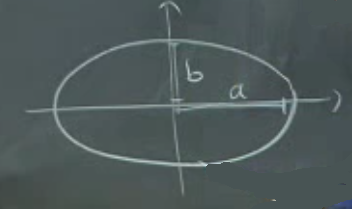
\includegraphics[height=2cm]{18_1.png}

\[ \bigg(\frac{x}{a}\bigg)^2 + \bigg(\frac{y}{b}\bigg)^2 = 1 \]

Formul cember formulune benziyor, tek fark $x,y$ kordinatlari farkli
sekillerde tekrar olceklenmisler (rescale). Elipsin alanini hesaplayalim. 

Diyelim ki 

\[ \int \int dx \ dy \]

olarak basladik. Ve

\[ \bigg(\frac{x}{a}\bigg)^2 + \bigg(\frac{y}{b}\bigg)^2 < 1 \]

olmak uzere $x,y$ uzerinden entegral alacagiz. Sinirlari ayarlamak,
vs. gibi islere hemen girisebiliriz, fakat bu is arap sacina donebilir. Bu
isi yapmanin en iyi yolu da degildir. 

Bu sekil bir cember olsaydi hemen kutupsal kordinata gecebilirdik, fakat
ustteki durumda bunu hemen yapamayiz. Fakat elips kenarlarindan bir basilmis
cemberdir, o zaman cemberi $a,b$ ile tekrar olceklersek, elips problemimizi
bir cember problemine indirgeyebiliriz. 

\[ \frac{x}{a} = u, \frac{y}{b} = v \]

O zaman alan soyle tanimlanabilir 

\[ \int \int_{u^2 + v^2 < 1} dx \ dy \]

Ama hala $dx,dy$ ile ne yapacagimiza karar vermedik. 

\[ du = \frac{1}{a}dx,dv = \frac{1}{b}dy \]

\[ du \ dv = \frac{1}{ab}dx \ dy \]

\[ dx \ dy = ab \ du \ dv \]

Entegrale sokarsak

\[ = ab \int \int_{u^2 + v^2 < 1} du \ dv \]

\[ = ab \cdot \textit{birim diskin alani} \]

\[ = \pi ab \]

Genel olarak yapmaya calistigimiz olcekleme faktorunun (scaling factor) ne
oldugunu bulmak, ki $dx \ dy$ ve $du \ dv$ arasindaki gecis mumkun olsun. 

Ornek 

\[ u = 3x - 2y \]

\[ v = x + y \]

Niye ustteki gibi $u,v$ kullanilmis? Belki entegre edilen fonksiyonu, belki
de sinirlari basitlestirmek istiyoruz. 

$dA = dx \ dy$, ya da $dA' = du \ dv$ 

Fakat bir problem var. Alan hesabinda entegralin ufak alan parcalarini
topladigini soylemistik. 

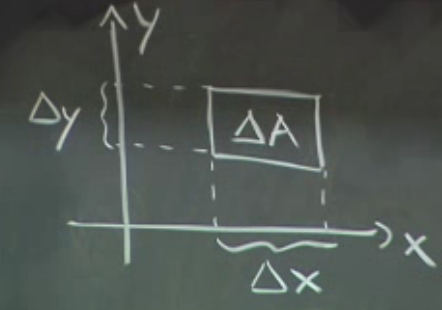
\includegraphics[height=2cm]{18_2.png}

Problem soyle, ustteki dikdortgen, bu ornegin donusum formullerine gore
$u,v$ baglaminda alttaki gibi bir sekle donusecek, yani paralelogram
olacak. 

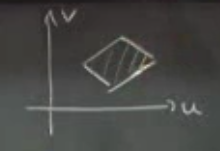
\includegraphics[height=2cm]{18_3.png}

Bir ornek uzerinde gorelim, her kenari 1 uzunlugunda, alani 1 olan kareyi
alirsak

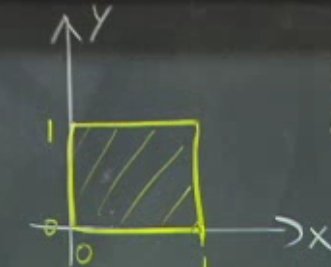
\includegraphics[height=3cm]{18_4.png}

ve bu karenin her noktasini $u,v$ formulleriyle donusturursek

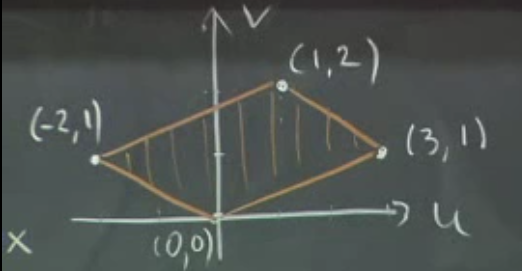
\includegraphics[height=3cm]{18_5.png}

elde edilir. Hakikaten bu bir paralelogram. Alan hesaplamak icin
determinant hesabi yapariz

\[ A' = 
\left|\begin{array}{rr}
3 & 1 \\
-2 & 1
\end{array}\right| = 5
 \]

$x,y$ formundaki 1 buyuklugundeki alan, 5 katina cikti. Yani 

\[ dA = 5 \ dA' \]

\[ du \ dv = 5 dx \ dy \]

O zaman entegrasyon sirasinda 

\[ \int \int ... \ dx \ dy = \int \int .. \ \frac{1}{5} du \ dv \]

haline gelmeli. 

Genel Durum 

\[ u = u(x,y) \]

\[ v = v(x,y)  \]

\[ \Delta u \approx u_x \Delta x + u_y \Delta y  \]

\[ \Delta v \approx v_x \Delta x + v_y \Delta y  \]

Matris formunda 

\[ 
\left[\begin{array}{r}
\Delta u \\
\Delta v 
\end{array}\right] \approx 
\left[\begin{array}{rr}
u_x & u_y \\
v_x & v_y
\end{array}\right] 
\left[\begin{array}{r}
\Delta x \\
\Delta y 
\end{array}\right] 
 \]

Demek ki kenarlari $\Delta x,\Delta y$ olan dikdortgen transform
edildiginde, kenarlari $\Delta u,\Delta v$ olan paralelogramin sekli kismi
turevlere bagli, cunku ustte transform eden matrisin icinde kismi turevler
var, ve kismi turevlerin degerleri belli $x,y$ noktalarinda hesaplandigina
gore, transformasyon ayrica belli $x,y$ noktalarina da bagli. Eger cebirsel
olarak turetseydik, alan buyuklugu olceklenmesinin (ustte 5 olan) ustteki
transform matrisinin determinanti oldugunu gorurduk. 

\[<\Delta x,0> \to <\Delta u, \Delta v> \approx <u_x \Delta x, v_x\Delta x> \]

\[ <0, \Delta y> \to <\Delta u,\Delta v> \approx <u_y\Delta y,v_y \Delta y> \]

Eger ustteki iki formulde sag taraftaki vektorlerin determinantini alirsak,
ki o vektorler paralelogramin kenarlaridir, o zaman 

\[ Alan' =  det(..)\Delta x \Delta y  \]

bulurduk. 

Degiskenin degisiminin Jacobian'i denen bir kavramdan bahsedelim simdi: 

\[ J = \frac{\partial (u,v)}{\partial(x,y)} \]

Bu cok garip bir notasyon. $\partial$ isareti kullaniyorum ama bu cercevede
kismi turev aldigim anlaminda degil, $du \ dv$ ve $dx \ dy$ arasindaki
orani hesapladigimi bana hatirlatmasi icin. 

\[ J =  \left|\begin{array}{rr}
u_x & u_y \\
v_x & v_y
\end{array}\right|
\]

O zaman 

\[ du \ dv = 
|J| dx \ dy = 
\bigg|\frac{\partial (u,v)}{\partial(x,y)}\bigg| dx \ dy
 \]

$|J|$ ifadesi Jacobian'in yani determinant hesabinin tam degeri (absolute
value) anlaminda. Eger $J$ sonucu mesela -10 cikarsa, biz 10 kullanacagiz. 

Ornek 

Kutupsal forma gecerken transformasyonun $r \ dr \ d\theta$ gerektirdigini
bir ornek uzerinden gormustuk. Simdi bu yeni metotu kullanarak ayni sonucu
bulmaya calisalim. 

\[  x= r cos\theta \]

\[  y= r sin\theta \]

Degisken degisiminin Jacoban'i

\[ J = \frac{\partial (x,y)}{\partial(r,\theta)}  =
\left|\begin{array}{rr}
x_r & x_\theta \\
y_r & y_\theta
\end{array}\right|   =
\left|\begin{array}{rr}
cos\theta & -rsin\theta\\
sin\theta & rcos\theta
\end{array}\right|
\]

En sagdaki determinanti hesaplayinca

\[ = rcos^2\theta + rsin^2\theta \]

\[ = r \]

O zaman 

\[ dx \ dy = |r| dr \ d\theta \]

$r$ her zaman pozitif olduguna gore tam deger isaretine gerek yok

\[ = r \ dr \ d\theta\]

Yorum 

$u,v$ orneginde hedef $J$ hesabinin bolum kismindaydi, simdi hedef
$r,\theta$ bolen kisminda. Bu problem olur mu? 

Olmaz, cunku 

\[ J = \frac{\partial (u,v)}{\partial(x,y)} \cdot
\frac{\partial (x,y)}{\partial(u,v)} = 1
 \]

yani $u,v \to x,y$ yonunde transformu yapan Jacobian ile $x,y \to u,v$
yonunde transform yapan Jacobian birbirinin tersi. Bu sebeple transformu
yaparken bu yonlerden hangisini hesapladiginiz onemli degil, en kolayi
hangisiyse onu hesaplayin, sonra eger ters yon gerekiyorsa $1 / sonuc$ ile
istediginiz sonucu elde edin. Zaten dikkat edilirse, $u,v$ transformunda
$|J|$, $dx,dy$ yaninda cikti, ustteki son ornekte $r$, $dr,d\theta$
yaninda. 

Ornek

\[ \int_0^1 \int_0^1 x^2y dx \ dy  \]

Aslinda bu hesabi oldugu gibi yapmak cok kolay. Fakat biz isi
zorlastirarak, degisken degisimi

\[ u =x  \]

\[ v = xy \]

sonrasi hesabi yapmaya ugrasacagiz. Bir degisken degisimi entegre edilen,
ya da sinir ifadelerini basitlestirmek icin yapilir, ama ustteki degisim
bunlari hicbirini yapmiyor. Sadece ornek amacli bu zor yolu sectik zaten. 

Once neyin entegre edildigini bulalim. 

1) Alan ogesini bulalim, Jacobian'i kullanalim. 

\[ \frac{\partial (u,v)}{\partial(x,y)}  = 
\left|\begin{array}{rr}
1 & 0 \\
y & x
\end{array}\right| = 
x
 \]

Yani

\[ du \ dv = x dx \ dy \]

Tabii $x$'in tam degeri olacak, ama tanimladigimiz sinir icinde zaten $x$
pozitif. 

2) Entegre edilen formulun $u,v$ iceren hali 

\[ x^2y dx \ dy =  x^2y  \frac{1}{x} du \ dv = 
xy du \ dv = 
v \ du \ dv 
\]
O zaman 

\[ \int \int _{???} v \ du \ dv \]

Yeni sinirlari bulalim. Ustteki entegrale bakalim, ic entegral $u$
degisiyor, $v$ sabit kaliyor demektir. O zaman $v=xy$ sabit demektir, her
sabit $xy$ icin alttaki resimdeki kirmizi cizgilerden biri dusunulebilir

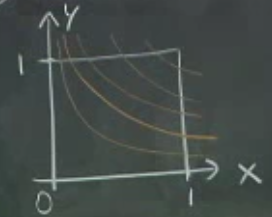
\includegraphics[height=3cm]{18_6.png}

Ic entegralin sinirlarini bulmak icin su soruyu cevaplamak gerekir, sabit
bir $v$ icin (cunku ic entegralde o sabit), $u$ degerleri hangi iki uc
deger arasinda hareket eder, ve entegrasyon bolgeme neresinden girip,
neresinden cikarim? 

Cevap icin tek bir kirmizi cizgiye bakarim, onun uzerinde giderken bolgeye
bir taraftan girip, oteki taraftan cikiyor olurum. 

Bolgenin en ust sinirini ele alalim, $y=1$. 

\[ y = \frac{v}{u}  \]

\[ u = v \]

O zaman $u$, $v$ ile ayni, $y=1$ iken hem $u,v$ 1'e esit.

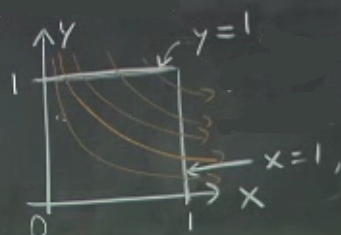
\includegraphics[height=3cm]{18_7.png}

Sinirin en ustunden basliyorum, $u$, $v$ ile ayni, kirmizi cizgiyi takip
ediyorum, ediyorum, asagi dogru inerken $u$ buyuyor. Sag kenardan disari
cikiyorum. Sag kenarda $x=1$, o zaman $u = 1$. Demek ki sinir

\[ \int \int _v^1 v \ du \ dv \]

Dis Entegral 

$v$'nin en az, en fazla degerleri alttaki resimde sari ile cizili

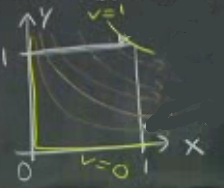
\includegraphics[height=4cm]{18_8.png}

\[ \int_0^1 \int _v^1 v \ du \ dv \]

Bu bizi bayagi zorladi. Ama eger bu yontem takip edilecekse, bazi
tavsiyeler, $u,v$ baglaminda kesitlerin ne oldugunu bulmak, sonra her
birinin ayri ayri uzerinde kalip bolgeye nereden girilip cikildigina
bakmak. 

Ise yaramazsa, o zaman tum bolge $u,v$ olarak cizilmeye
ugrasilabilir. Teker teker 

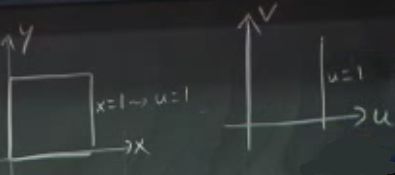
\includegraphics[height=3cm]{18_9.png}

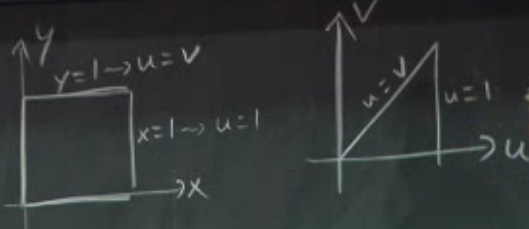
\includegraphics[height=3cm]{18_10.png}

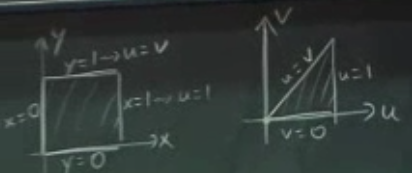
\includegraphics[height=3cm]{18_11.png}

$u,v$ baglaminda bir ucgen elde edildi, ve bu ucgen uygun sekilde kesilerek
cift entegral hesaplanabilir. 


















\end{document}
